\documentclass[a4paper,10pt]{article}

\usepackage{fullpage}
\usepackage[light]{antpolt}
\usepackage{todonotes}
\usepackage{listings}

% Setup for code snippets
\lstset{language=Python}
\lstset{frame=lines}
\lstset{label={lst:code_direct}}
\lstset{basicstyle=\footnotesize}

\begin{document}

\title{NaturalSelection: A Python package for user-friendly evolution of neural networks and others}
\author{Dan Saattrup Nielsen}
\date{\today}
\maketitle

\abstract{
  Hyperparameter optimisation of neural networks is an incredibly time consuming process. A grid search is usually too time consuming, and a random search does base its search on prior results and is therefore still wasteful. Other approaches include Bayesian optimisation and genetic algorithms, both of which are ``guided'', meaning that they base the choice of hyperparameters on past performance. We propose a new Python package, NaturalSelection, which provides a simple Pythonic API for applying genetic algorithms to general optimisation problems, with built-in support for tuning both the hyperparameters and architecture of neural networks. Several other Python packages that optimise hyperparameters of neural networks exist, but these are utilising algorithms that tune the hyperparameters not including the architecture, such as learning rate, momentum and batch size. Our package ``evolves'' a neural network, starting from a shallow network and gradually making it more complex while optimising performance. As a side benefit this prioritises simpler neural architectures, resulting in faster training times.
}

\section{Example}

Here is an example of finding a multilayer perceptron to model the well-known dataset Fashion-MNIST. Here the \textsf{fashion\_mnist\_train\_val\_sets} function fetches the dataset and performs standard normalisation preprocessing.

\lstset{caption = Evolution of a population of MLPs on Fashion-MNIST}
\begin{lstlisting}
  >>> import naturalselection as ns
  >>>
  >>> nns = ns.NNs(
  ...   size = 20,
  ...   train_val_sets = fashion_mnist_train_val_sets(),
  ...   loss_fn = 'categorical_crossentropy',
  ...   score = 'accuracy',
  ...   output_activation = 'softmax',
  ...   max_epochs = 1,
  ...   max_training_time = 120,
  ...   )
  ...
  >>> history = nns.evolve(generations = 20)
  Evolving population: 100%|===================| 20/20 [1:32:00<00:00, 73.22s/it]
  Computing fitness: 100%|=======================| 11/11 [05:37<00:00, 22.52s/it]
  >>> 
  >>> history.fittest
  {'genome': {'optimizer': 'adamax', 'hidden_activation': 'relu',
  'batch_size': 32, 'initializer': 'glorot_uniform', 'input_dropout': 0.0,
  'neurons0': 256, 'dropout0': 0.3, 'neurons1': 512, 'dropout1': 0.3,
  'neurons2': 128, 'dropout2': 0.0, 'neurons3': 0, 'dropout3': 0.1,
  'neurons4': 1024, 'dropout4': 0.2}, 'fitness': 0.855400025844574}
\end{lstlisting}

\pagebreak
From the evolved population we can then plot the evolution.
\lstset{caption = Plotting the evolution}
\begin{lstlisting}
  >>> history.plot(
  ...   title = "Validation accuracy by generation",
  ...   ylabel = "Validation accuracy"
  ...   )
\end{lstlisting}

\begin{center}
  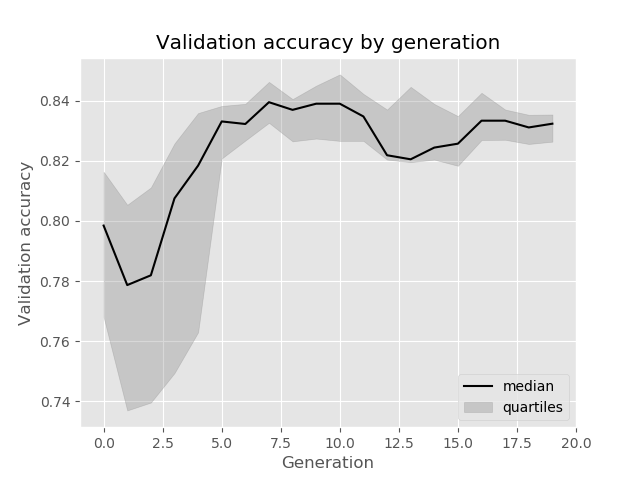
\includegraphics[scale=0.5]{gfx/fashion_mnist_example.png}
\end{center}

Lastly, we can train the best performing model and save it locally:

\lstset{caption = Saving the model with the optimised hyperparameters}
\begin{lstlisting}
  >>> # Training the best model and saving it to fashion_mnist_model.h5
  >>> best_score = nns.train_best(file_name = 'fashion_mnist_model')
  Epoch 0 - val_acc: 0.853: 100%|=========| 60000/60000 [00:21<00:00, 146.25it/s]
  (...)
  Epoch 44 - val_acc: 0.900: 100%|========| 60000/60000 [00:21<00:00, 284.68it/s]
  >>>
  >>> best_score
  0.9029
\end{lstlisting}

\end{document}
